%%%%%%%%%%%%%%%%%%%%%%%%%%%%%%%%%%%%%%%%%
% Short Sectioned Assignment
% LaTeX Template
% Version 1.0 (5/5/12)
%
% This template has been downloaded from:
% http://www.LaTeXTemplates.com
%
% Original author:
% Frits Wenneker (http://www.howtotex.com)
%
% License:
% CC BY-NC-SA 3.0 (http://creativecommons.org/licenses/by-nc-sa/3.0/)
%
%%%%%%%%%%%%%%%%%%%%%%%%%%%%%%%%%%%%%%%%%

%----------------------------------------------------------------------------------------
%	PACKAGES AND OTHER DOCUMENT CONFIGURATIONS
%----------------------------------------------------------------------------------------

\documentclass[paper=a4, fontsize=11pt]{scrartcl} % A4 paper and 11pt font size
\usepackage[brazilian]{babel}
\usepackage[utf8]{inputenc}
\usepackage[T1]{fontenc}
\usepackage{amsmath,amsfonts,amsthm,mathtools} % Math packages
\usepackage{xspace}
\usepackage{indentfirst}
\usepackage{placeins}
\usepackage{hyperref}

\usepackage{tikz}
\usetikzlibrary{arrows}
\usetikzlibrary{positioning}
\usetikzlibrary{calc}

%\usepackage{sectsty} % Allows customizing section commands
%\allsectionsfont{\centering \normalfont\scshape} % Make all sections centered, the default font and small caps

\usepackage{fancyhdr}
\pagestyle{fancyplain}
%\fancyhead{}
\fancyfoot[L]{} % Empty left footer
\fancyfoot[C]{} % Empty center footer
\fancyfoot[R]{\thepage} % Page numbering for right footer
\renewcommand{\headrulewidth}{0pt} % Remove header underlines
\renewcommand{\footrulewidth}{0pt} % Remove footer underlines
\setlength{\headheight}{13.6pt} % Customize the height of the header

\bibliographystyle{apalike}

%\sectionfont{\bfseries\Large\raggedright}
%\subsectionfont{\bfseries\Large\raggedright}

\newtheorem{theorem}{Teorema}
\newtheorem{definition}{Definição}
\newtheorem{property}{Propriedade}
\newtheorem{proposition}{Proposição}

\newenvironment{example}[1][Exemplo]{\begin{trivlist}
\item[\hskip \labelsep {\bfseries #1}]}{\end{trivlist}}
\newenvironment{exerc}[1][Exercício]{\begin{trivlist}
\item[\hskip \labelsep {\bfseries #1}]}{\end{trivlist}}


\numberwithin{equation}{subsection}
\numberwithin{figure}{subsection}
\numberwithin{table}{subsection}
\numberwithin{definition}{subsection}
\numberwithin{theorem}{subsection}
\numberwithin{property}{subsection}
\numberwithin{proposition}{subsection}
%\numberwithin{example}{subsection}

\numberwithin{equation}{section}
\numberwithin{figure}{section}
\numberwithin{table}{section}
\numberwithin{definition}{section}
\numberwithin{theorem}{section}
\numberwithin{property}{section}
\numberwithin{proposition}{section}
%\numberwithin{example}{section}

\def\ind{\perp\!\!\!\perp}
\def\nind{\not\!\perp\!\!\!\perp}

% Default fixed font does not support bold face
\DeclareFixedFont{\ttb}{T1}{txtt}{bx}{n}{12} % for bold
\DeclareFixedFont{\ttm}{T1}{txtt}{m}{n}{12}  % for normal

% Custom colors
\usepackage{color}
\definecolor{deepblue}{rgb}{0,0,0.5}
\definecolor{deepred}{rgb}{0.6,0,0}
\definecolor{deepgreen}{rgb}{0,0.5,0}

\usepackage{listings}

\definecolor{mygreen}{rgb}{0,0.6,0}
\definecolor{mygray}{rgb}{0.5,0.5,0.5}
\definecolor{mymauve}{rgb}{0.58,0,0.82}

\lstset{ %
  backgroundcolor=\color{white},   % choose the background color
  basicstyle=\ttfamily\normalsize,        % size of fonts used for the code
  breaklines=true,                 % automatic line breaking only at whitespace
  captionpos=b,                    % sets the caption-position to bottom
  commentstyle=\color{mygreen},    % comment style
  escapeinside={\%*}{*)},          % if you want to add LaTeX within your code
  keywordstyle=\color{blue},       % keyword style
  stringstyle=\color{mymauve},     % string literal style
}

% Python environment
\lstnewenvironment{python}[1][]
{
\pythonstyle
\lstset{#1}
}
{}


%\setlength{•}{•}\parindent{0pt} % Removes all indentation from paragraphs - comment this line for an assignment with lots of text

%----------------------------------------------------------------------------------------
%	TITLE SECTION
%----------------------------------------------------------------------------------------

\newcommand{\horrule}[1]{\rule{\linewidth}{#1}} % Create horizontal rule command with 1 argument of height

\title{	
\normalfont \normalsize 
\textsc{Modelos Probabilísticos Baseados em Grafos} \\ 
\textsc{Prof. Denis Mauá} \\ [25pt]
%\horrule{0.5pt} \\[0.4cm] % Thin top horizontal rule
\huge Eliminação de Variáveis em\\ Redes de Markov [25pt]
%\horrule{1pt} \\[0.5cm] % Thick bottom horizontal rule
}
\author{Thales A. B. Paiva \\ thalespaiva@gmail.com} % Your name
\date{\today} % Today's date or a custom date

\renewcommand{\P}{\mathbb{P}}
\renewcommand{\bar}[1]{\overline{#1}}
\newcommand{\set}[1]{\mathcal{#1}}

\begin{document}


\maketitle % Print the title
\horrule{1pt} \\[0.5cm] % Thick bottom horizontal rule

\tableofcontents

\pagebreak
\section{Implementação dos algoritmos em Python}

Foi pedido que implementássemos o algoritmo de eliminação de variáveis, e algumas heurísticas para determinar a ordem da eliminação. 

\section{Eliminação de Variáveis}

Implementei a eliminação de variáveis como um método da classe \verb|Potential|, do módulo \verb|distribution.py| que trata dos potenciais. Esta classe tem a seguinte interface:

\begin{lstlisting}[language=python]
class Potential:
    def __init__(self, scope, values=None)
    def has_variable(self, variable)
    def __str__(self)
    def __getitem__(self, key)
    def __setitem__(self, key, value)
    def set_values(self, values)
    def evaluate(self, var_valuation)
    def __mul__(self, himself)
    def __mod__(self, variable)
    def __truediv__(self, probab)
    def normalize(self)
    def combine(potentials)
    def eliminate_variables(potentials_tuple, variables)
\end{lstlisting}


O método \verb|eliminate_variables| é implementação direta do algoritmo descrito nas salas de aula. Pode ser visto abaixo. Note que a eliminação de uma variável é feita como \verb|Pot2 = Pot1 % var|. O método \verb|combine| toma uma lista de potenciais e devolve sua combinação, ou seja, o produto entre todos eles.

\begin{lstlisting}[language=python]
    def eliminate_variables(potentials_tuple, variables):
        potentials = list(potentials_tuple)

        for variable in variables:
            dependents = []
            for pot in potentials:
                if pot.has_variable(variable):
                    dependents.append(pot)
            combined = Potential.combine(dependents)
            for dep in dependents:
                potentials.remove(dep)
            potentials.append(combined % variable)

        return Potential.combine(potentials)
\end{lstlisting}

\subsection{Exemplo}

Para a rede de Markov \verb|grid3x3.uai| da UAI Inference Competition, temos a seguinte rede (desenhada com o método \verb|MarkovNet.draw|.

\begin{figure}[hbtp]
\centering
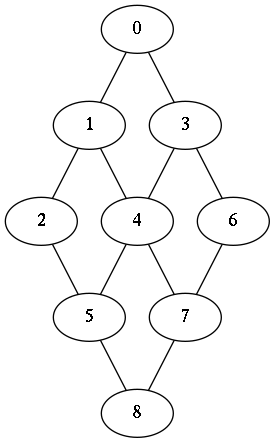
\includegraphics[scale=0.7]{images/grid3x3.png}
\caption{Rede de Markov \texttt{grid3x3}.}
\label{fig:alcanc}
\end{figure}


Podemos calcular a função de partição usando a eliminação de variáveis pelo método \verb|MarkovNet.get_partition_function|.

\begin{lstlisting}[language=python]
def get_partition_function(self, evidence={}):
  variables = self.variables.values()
  non_evid_vars = ([v for v in variables if v.name not in evidence])
  potentials = tuple(self.potentials.values())

  reduced = Potential.eliminate_variables(potentials, non_evid_vars)
  return reduced.evaluate(evidence)
\end{lstlisting}

Para o arquivo de evidência dado na competição, temos:
\begin{verbatim}
$ python -m programods.markovnet examples/markovnet/grid3x3/grid3x3.uai 
    examples/markovnet/grid3x3/grid3x3.uai.evid 
partition function log10 for evid  1: 14.889867
\end{verbatim}

Que é exatamente o esperado.

\section{Ordem de Eliminação}

Para determinar a ordem de eliminação, implementei 3 heurísticas:
\begin{itemize}
  \item \textsc{MinFill};
  \item \textsc{MinDegree};
  \item \textsc{WeightedMinFill}.
\end{itemize}

Todas elas são implementadas como métodos da classe \verb|MarkovGraph|. Esta classe tem a interface declarada abaixo.
\begin{lstlisting}[language=python]
class MarkovGraph():
    def __init__(self, adjacencies=None):
    def variables(self):
    def __getitem__(self, key):
    def __setitem__(self, key, value):
    def __iter__(self):
    def __delitem__(self, key):
    def get(self, key, failed_return_value):
    def gen_graph(markov_net, variables=None):
    def get_reduced_copy(self, variables=None):
    def draw(self, file_path, variables=None):
    def get_min_fill_variable(self):
    def get_min_degree_variable(self):
    def get_weighted_min_fill_variable(self):
    def get_elimination_ordering_by_min_fill(self, elim_variables=None):
    def get_elimination_ordering_by_min_degree(self, elim_variables=None):
    def get_elimination_ordering_by_weighted_min_fill(self, elim_variables=None):
    def get_elimination_ordering_by_heuristic(self, heuristic_select, elim_variables=None):
    
\end{lstlisting}


Para evitar código repetido, imeplementei um método \verb|get_elimination_ordering_by_heuristic| que recebe uma heurística de seleção e as variáveis para eliminar. Quando não é passada nenhuma variável para eliminar, ele elimina todas (o que escrito assim parece um pouco estúpido, mas achei útil na hora de usar).
\begin{lstlisting}[language=python]
    def get_elimination_ordering_by_heuristic(self, heuristic_select, elim_variables=None):

        if elim_variables is None:
            variables = list(self.variables.values())
        else:
            variables = list(elim_variables)

        graph = self.get_reduced_copy(variables)
        ordering = []
        for _ in range(len(variables)):
            selected_variable = heuristic_select(graph)

            for neighbor in graph[selected_variable]:
                adjacent = graph[neighbor] | graph[selected_variable]
                graph[neighbor] = adjacent - {neighbor, selected_variable}

            del graph.adjacencies[selected_variable]
            variables.remove(selected_variable)
            ordering.append(selected_variable)

        return ordering
\end{lstlisting}

As implementações das heurísticas de seleção são dadas a seguir.

\subsection{MinFill};

\begin{lstlisting}[language=python]
    def get_min_fill_variable(self):
        min_fill = None
        min_fill_var = None

        def get_n_fill_edges_on_elimination(variable):
            neighbors = self[variable]
            n_edges = 0
            for neighbor in neighbors:
                n_edges += len(self[neighbor] & neighbors)

            return (len(neighbors) * (len(neighbors) - 1) - n_edges) // 2

        for variable in self:
            fill = get_n_fill_edges_on_elimination(variable)
            if min_fill is None or fill < min_fill:
                min_fill = fill
                min_fill_var = variable

        return min_fill_var
\end{lstlisting}

\subsection{MinDegree};

\begin{lstlisting}[language=python]
    def get_min_degree_variable(self):
        min_degree = None
        min_degree_var = None

        for variable in self:
            degree = len(self[variable])
            if min_degree is None or degree < min_degree:
                min_degree = degree
                min_degree_var = variable

                return min_degree_var
\end{lstlisting}

\subsection{WeightedMinFill}.

\FloatBarrier
\begin{lstlisting}[language=python]
    def get_weighted_min_fill_variable(self):
        min_fill = None
        min_fill_var = None

        def get_weighted_fill_edges_on_elimination(variable):
            neighbors = self[variable]
            weighted_fill = 0
            for neighbor in neighbors:
                for common_friend in self[neighbor] & neighbors:
                    weighted_fill += (neighbor.cardinality *
                                      common_friend.cardinality)
            return weighted_fill // 2

        for variable in self:
            fill = get_weighted_fill_edges_on_elimination(variable)
            if min_fill is None or fill < min_fill:
                min_fill = fill
                min_fill_var = variable

        return min_fill_var
\end{lstlisting}


\section{Eficiência}

A Tabela~\ref{tab_exec} mostra alguns valores do tempo de execução para as entradas \verb|Grid3x3| e \verb|Grid4x4|. Podemos ver como o algoritmo de enumeração rapidamente se torna inviável. O \textsc{MinDegree} e o \textsc{WeightedMinFill} se saem pior no grid 4 por 4, provavelmente por causa da minha implementação. Isso pois, como uso a conjuntos, calcular é reduzido a calcular o tamanho de interseções. Do modo como implementei, também foi inviável tratar de arquivos de entrada muito grande. Estou trabalhando em melhorar isso.
\begin{table}[]
\centering
\caption{Tempo de execução}
\label{tab_exec}
\begin{tabular}{lll}
\textbf{Algoritmo}          & \textbf{\texttt{Grid3x3}}   & \textbf{\texttt{Grid4x4}}   \\
\textsc{Enumeration}        & 23.2 ms                     & 5.87 s                      \\
\textsc{MinFill}            & 1.53 ms                     & 4.82 ms                     \\
\textsc{MinDegree}          & 1.79 ms                     & 14.3 ms                     \\
\textsc{WeightedMinFill}    & 1.79 ms                     & 5.48 ms                                             
\end{tabular}
\end{table}
\end{document}
